\part{Capitulo 4}
\vspace{-0.3cm}
\begin{center}
    \begin{large}
        Metodos Probabilisticos y Estadisticos
    \end{large}
\end{center}

La mayor parte de los procesos hidrologicos son aleatorios, no existen procesos puramente deterministicos. En consecuencia, para poder hacer una caracterizacion se \textbf{debe registrar la ocurrencia de ellos} mediante registros historicos, los cuales son sometidos a un post procesado estadistico.
\\ \\
Los objetivos son los siguientes:

\begin{itemize}
    \item Estimacion de P( ) de que ocurra un determinado evento
    \item Estimacion de eventos que no han ocurrido o no se han observado
    \item Caracterizacion estadistica de series hidrologicas
    \item Correlacion y regrecion para completar y extender series
\end{itemize}

\section{Frecuencia Relativa y Acumulada}

La sumatoria de todas las frecuencias relativas debe ser igual a 1, es decir:

\begin{equation}
    \sum_{i=1}^{n} f_i = 1
\end{equation}

Estas funciones son obtenidas a partir de una muestra, por lo que se pueden obtener de estimaciones de la poblacion aproximando como limites:

\begin{figure}[H]
    \centering
    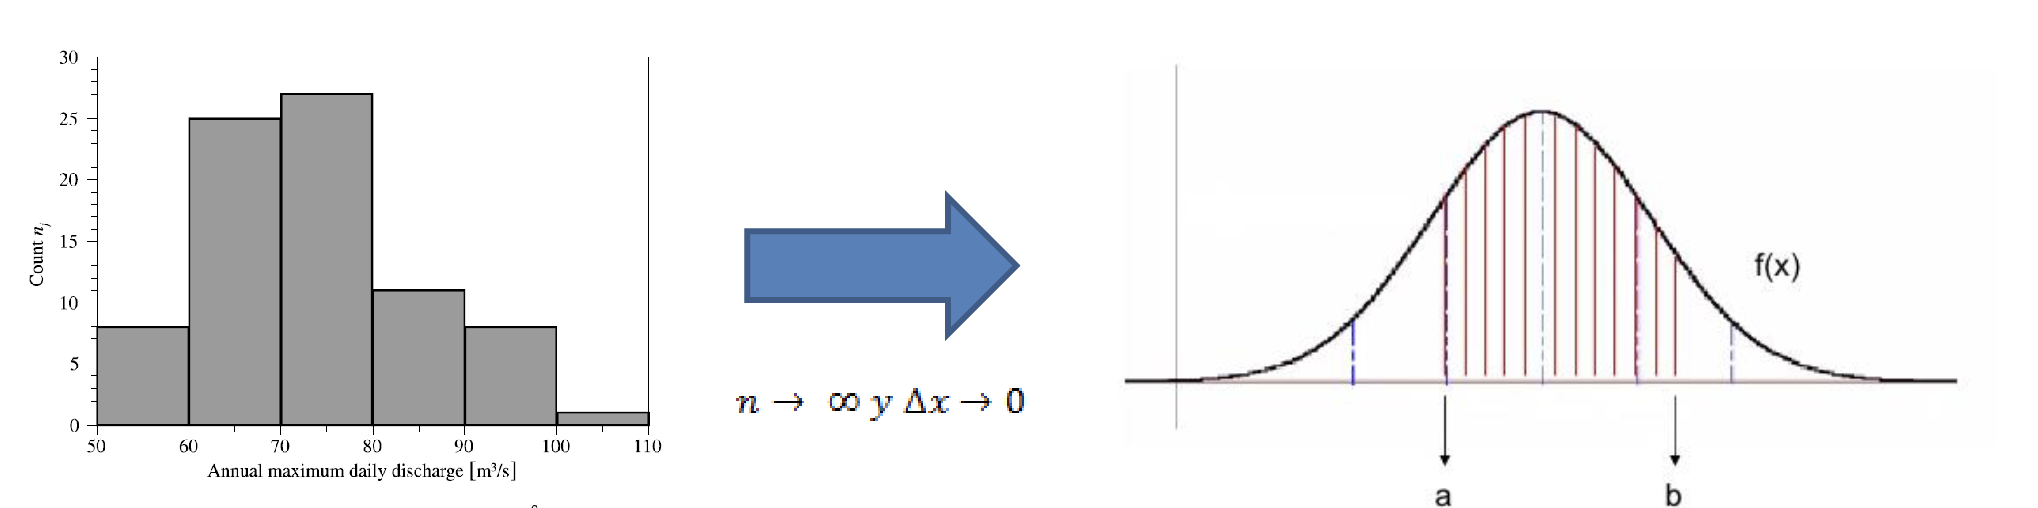
\includegraphics[width=0.85\textwidth]{imagenes/frecuencia.png}
    \label{fig:frecuencia_acumulada}
\end{figure}

\section{Periodo de Retorno y P( ) de Excedencia}

Se puede definir como: el intervalo de recurrencia promedio entre evnetos que igualan o excedan una magnitud especifica
\\ \\
Es decir, en un horizonte de tiempo grande, se esperaria observar eventos iguales o mayores cada \textbf{T años}.
\\ \\
Sea \textbf{p} la probabilidad de exito y \textbf{(1-p)} la probabilidad de falla en un determinado año. Podemos definir la \textbf{probabilidad de recurrencia $\pi$} como el producto de \textbf{$\pi$ - 1} fallas seguidas por un exito, por lo tanto:

\begin{equation}
    P(X > X_t) = \frac{1}{T}
\end{equation}

Ejemplo:

\begin{figure}[H]
    \centering
    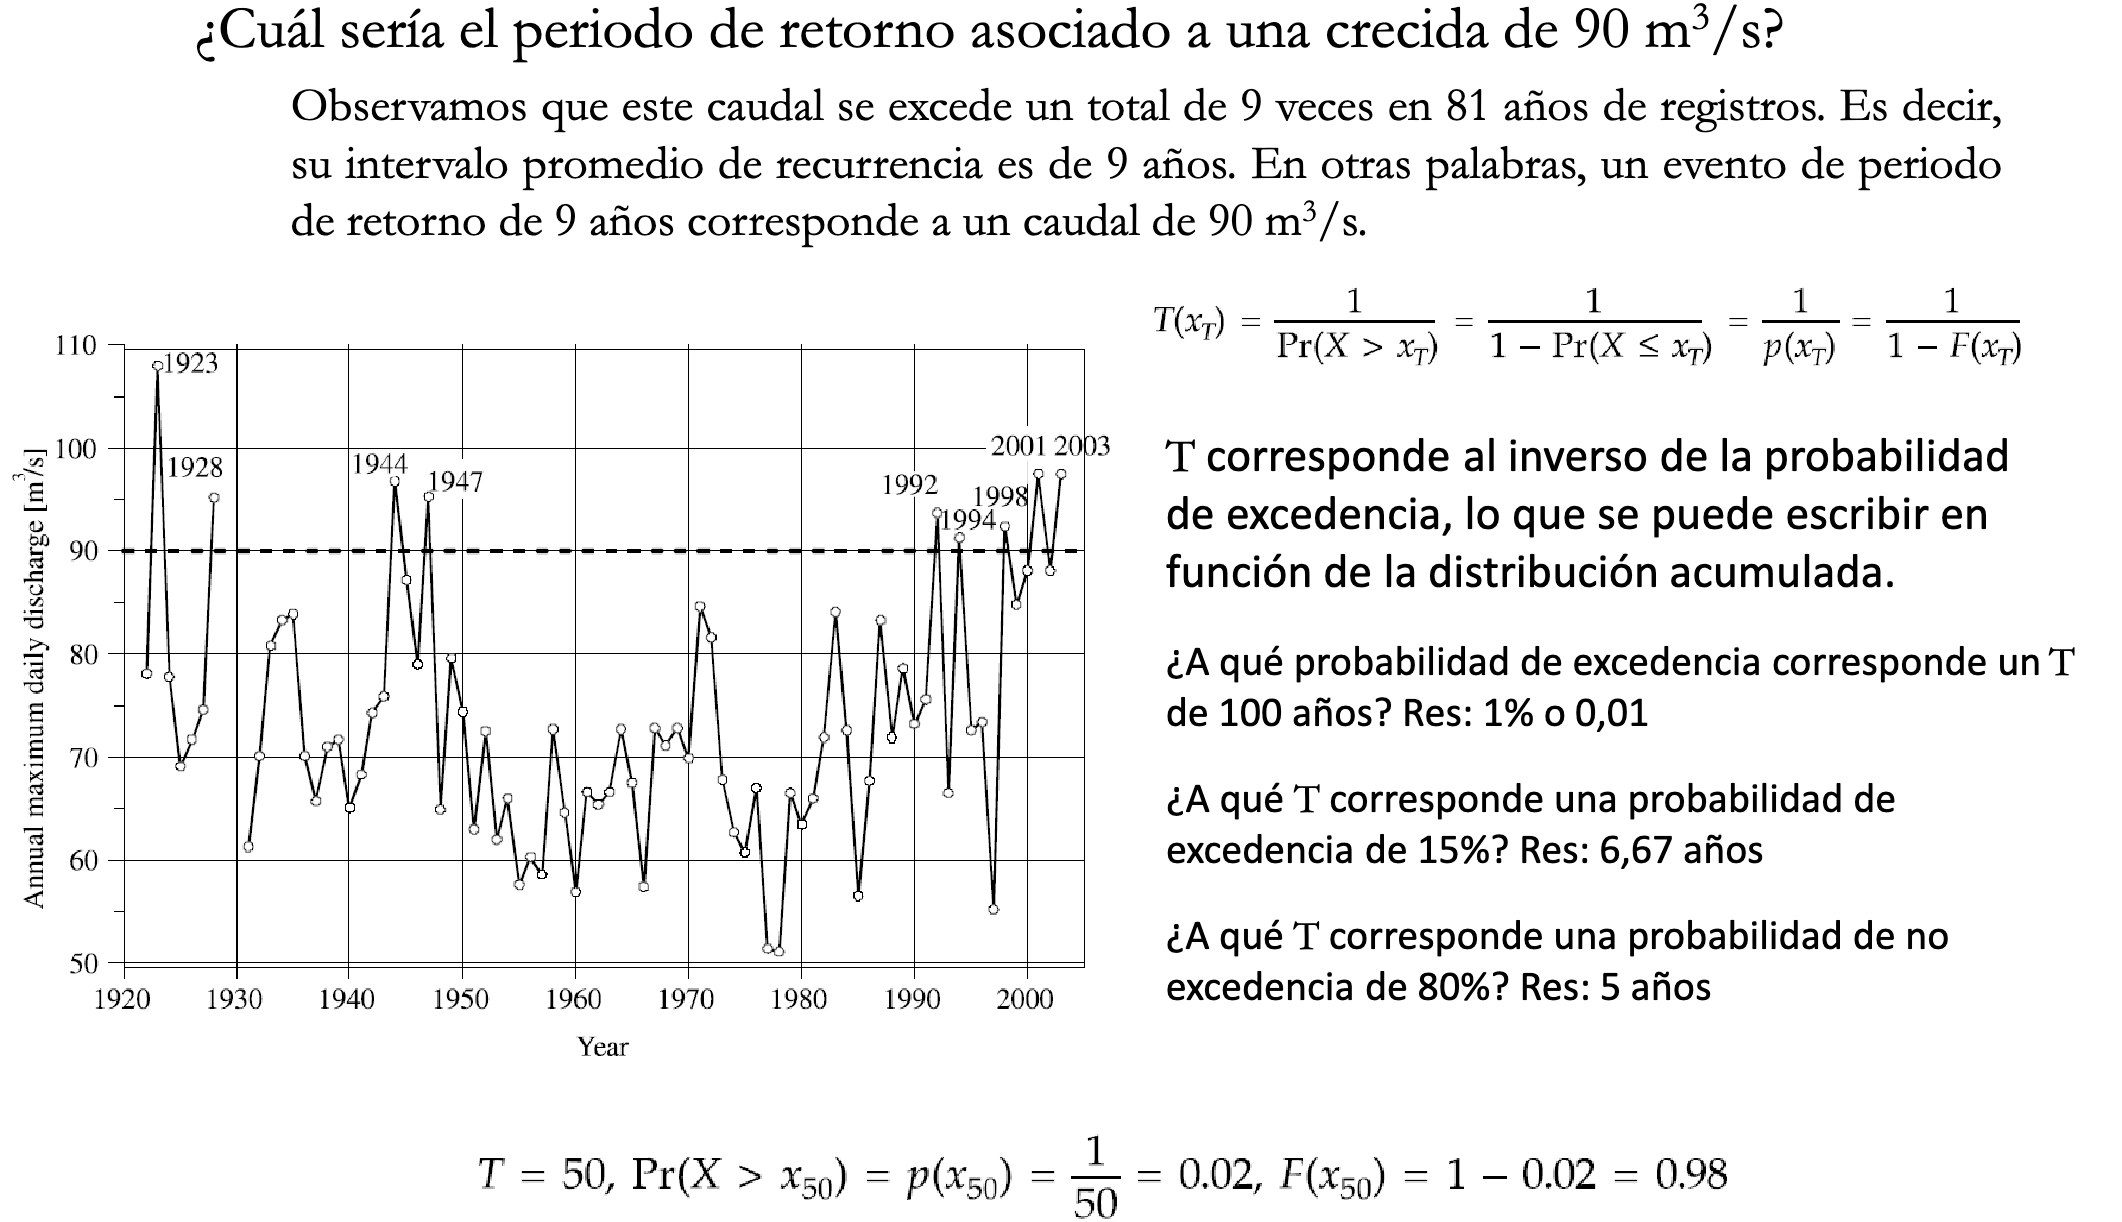
\includegraphics[width=0.85\textwidth]{imagenes/retorno.png}
    \label{fig:periodo_retorno}
\end{figure}

\section{Seguridad y Riesgo Hidrololgico}

Se define como la probabilidad de no excedencia:

\begin{equation}
    P_{no-exc} = 1 - \frac{1}{T}
\end{equation}

Por lo tanto, la probabilidad de que cierto valor no se exceda en n años es:

\begin{equation}
    S = (1 - \frac{1}{T})^n 
\end{equation}

Lo cual se define como \textbf{Seguridad Hidrologica}, donde su complemento es el \textbf{Riesgo Hidrologico}, lo cual se usa para obras hidraulicas:

\begin{eqnarray}
    R = 1- S = 1 - (1 - \frac{1}{T})^n
\end{eqnarray}

